
% Many thanks to Andrew West for writing most of this file
% Main LaTeX file for CIS400/401 Project Proposal Specification
%
% Once built and in PDF form this document outlines the format of a
% project proposal. However, in raw (.tex) form, we also try to
% comment on some basic LaTeX technique. This is not intended to be a
% LaTeX tutorial, instead just (1) a use-case thereof, and (2) a
% template for your own writing.

% Ordinarily we'd begin by specifying some broad document properties
% like font-size, page-size, margins, etc. -- We have done this (and
% much more) for you by creating a 'style file', which the
% 'documentclass' command references.
\documentclass{sig-alternate}
 
% These 'usepackage' commands are a way of importing additional LaTeX
% styles and formattings that aren't part of the 'standard library'
\usepackage{mdwlist}
\usepackage{url}

\begin{document} 

% We setup the parameters to our title header before 'making' it. Note
% that your proposals should have actual titles, not the generic one
% we have here.
\title{CodeScore}
\subtitle{Dept. of CIS - Senior Design 2013-2014\thanks{Advisor: Chris Murphy (cdmurphy@cis.upenn.edu).}}
\numberofauthors{4}

\author{
Allison Pearce \\ \email{alpearce@upenn.edu} \\ Univ. of Penn \\ Philadelphia, PA
\and Spencer Lee \\ \email{lesp@upenn.edu} \\ Univ. of Penn \\ Philadelphia, PA
\and Tanvir Ahmed \\ \email{tanvir@upenn.edu} \\ Univ. of Penn \\ Philadelphia, PA
\and Will McDermid \\ \email{wmcd@upenn.edu} \\ Univ. of Penn \\ Philadelphia, PA}

\date{}
\maketitle

% Next we write out our abstract -- generally a two paragraph maximum,
% executive summary of the motivation and contributions of the work.
\begin{abstract}
  \textit{The technology industry lacks automated tools for evaluating software quality. These tools would be helpful for individuals desiring to improve their abilities, recruiters searching for top programmers, and educators needing to quickly assess student performance. We propose to develop an application that calculates a metric for internal quality by detecting code smells, easily recognized design weaknesses that may indicate more significant problems within the system. The program will recognize code smells using a set of specific rules. It will then use the results to compute a CodeScore: a single value that reflects the maintainability and understandability of the piece of software based on the presence of code smells. }
\end{abstract}

% Then we proceed into the body of the report itself. The effect of
% the 'section' command is obvious, but also notice 'label'. Its good
% practice to label every (sub)-section, graph, equation etc. -- this
% gives us a way to dynamically reference it later in the text via the
% 'ref' command.
\section{Introduction}
\label{sec:intro}
Software failures result in annoyed users at best, and they can cause catastrophic system failures at worst. Six people received massive radiation overdoses from a radiation therapy device in one of the canonical examples of a fatal software error \cite{leveson1995therac}. Failures are consequences of poor software quality. Software quality is defined as ``conformance to explicitly stated functional and performance requirements, explicitly documented development standards, and implicit characteristics that are expected of all professionally developed software" \cite{pressman1997}. In addition to causing failures, disregard for software quality is expensive and inefficient, requiring more dollars and man-hours to maintain, test, and add features to project than should be necessary. An increasing appreciation of well-designed software has been manifested in the international standard for software quality, ISO/IEC 25010. The standard affirms the importance of specifying and measuring characteristics of quality, and it defines quality models intended to aid in accomplishing these goals [cite this].

Software quality is commonly divided into internal quality and external quality. External quality describes how well the software meets performance expectations, and encompasses characteristics such as correctness, accuracy, integrity, robustness, reliability, usability, adaptability, and efficiency. Internal quality describes how well the software was designed and implemented, and is concerned with maintainability, flexibility, portability, reusability, readability, understandability, and testability \cite{mcconnell1993codecomplete}. Internal and external quality are closely related, and deficiencies in internal quality lead to deficiencies in external quality. For example, code that is difficult to understand will also be difficult to adapt to new requirements, and code that cannot be easily tested will likely be incorrect or unreliable. 


%projects bigger -> quality more important
%costs in terms of time, efficiency, monies, man-hours

One way to diagnose internal quality issues is by detecting code smells. Code smells are easily recognized design weaknesses that may indicate deeper, more significant problems within the system. Some common code smells include:
\begin{itemize}
\item Classes or methods that have too many lines of code
\item Duplicated code
\item Long lists of parameters for functions
\item Overly complex conditional logic
\item Inconsistent or uncommunicative naming conventions
\end{itemize}

Individual code smells are directly related to problems with specific aspects of internal quality. For example, overly complex conditional logic and inconsistent naming conventions hurt understandability and readability. Duplicated code implies that changes will have to be made not once but everywhere that the duplication occurs, which hurts maintainability. 

The proposed application tests for the presence of code smells in order to evaluate internal quality. We will define rules for custom algorithms to detect code smells, and the results of the detection will be used compute an internal quality score for a code sample. The program focuses specifically on how code smells relate to two elements of internal software quality, maintainability and understandability. These elements are underemphasized in most classroom settings. Students work quickly and haphazardly to meet deadlines and never revisit their program after turning it in, so there is no need to write maintainable or understandable code.  However, understandability and maintainability are critical outside of the classroom, where teams of developers need to understand code they did not write, and to maintain it for years as the product evolves. The proposed tool will help students assess and improve these necessary software engineering skills by providing objective feedback to make them aware of their weaknesses. Computer science teachers can use the the application when grading assignments to assess quality without spending hours reading through each student's source code. It will also allow recruiters to identify potential employees who will contribute to their company's products with a high regard for quality. Overall, this tool will help the technology industry to train and recruit a strong developer workforce who will write programs that are internally sound. 

\section{Related Work}
\label{sec:related_work}
In this section, we will provide background information on the different methods of analyzing code, the standards for measuring code quality, and various services and applications that already strive to provide quantitative analyses of code quality.


\subsection{Code Analysis Methodologies}
The majority of existing applications for measuring code quality rely on well-established code analysis techniques. These techniques involve breaking code down into specific units and measuring the counts of these units. Such techniques include parsing the source code into control structures \cite{mccabe1976complexity}, tokens \cite{halstead1977elements}, assembly instructions \cite{park1992software}, or objects \cite{chidamber1994metrics}. Once the source code has been parsed into some unit (this process is called static analysis), the attributes of the code, such as reliability, security, efficiency, size, and maintainability can be measured from the parsed results. The actual approach to measuring these attributes originated in \cite{boehm1976quantitative} and later became part of the ISO/IEC 25000 series of standards relating to the quality and evaluation of software \cite{iso2011iec}. These techniques and standards comprise the foundation for today's code quality measurement applications, and they will be the basis for our approach as well.

\subsection{Ohloh}
Launched in January of 2006, Ohloh \cite{allen2009ohloh} is web service and online community owned by Black Duck Software which provides basic metrics for over 650,000 open source projects containing over 24,000,000,000 lines of code located in over 620,000 source code repositories and managed by more than 3,000,000 contributors. These projects are retrieved from source control repositories and analyzed. Metrics such as lines of code, amount of source code comments, and estimated software cost (based on the COCOMO model \cite{boehm2000software}) are provided, along with commit statistics, project activity, and programming language detection. This data is graphically displayed when one views a project's information on the site. Ohloh also provides global statistics across all projects for different programming languages and contributor statistics for different authors of open source code. 

Ohloh primarily focuses on tracking project/contributor activity for large open-source projects. Our proposed application will focus more on providing code quality-oriented metrics.

\subsection{Common Weakness Enumeration}
The Common Weakness Enumeration (CWE) \cite{mitre2006cwe} is a community-developed list of software weaknesses hosted by the MITRE Corporation. The CWE was developed with the intention of providing:

\begin{itemize}
\item a common standard of identifying, mitigating, and preventing software weaknesses.
\item a common source of measuring weaknesses for software security tools.
\item a common language for describing the various types of software weaknesses that exist in computer architecture, software design, and source code.
\end{itemize}

CWE supports the discovery of common types of software security flaws such as buffer overflows, handler errors, pathname traversals, and resource management errors (amongst others) within code.

CWE began with the Common Vulnerabilities and Exposures (CVE) list in 1999 \cite{mitre2005cve}. As part of the SAMATE project \cite{nist2005samate}, MITRE later expanded upon the CVE list with the Preliminary List of Vulnerability Examples for Researchers (PLOVER) \cite{christey2005plover}. PLOVER was the first attempt to take real-world examples of software vulnerabilities and abstract them into common classes of more general vulnerabilities that can arise during the software development process. The goal of PLOVER was to make this information available to developers, researchers, and analysts so that they may use it for a variety of purposes, with the goal of improving code security. CWE encompasses much of the CVE list and expands upon PLOVER by establishing community-developed definitions and descriptions of these common weaknesses.

CWE, though possibly a valuable resource for our endeavors, primarily strives to provide standards relating to the weaknesses of code in terms of security. This may be a valuable resource for our proposed application, as many code weaknesses are indicative of, or are themselves, code smells.

\subsection{Other Static Code Analysis Tool}
A wide variety of other static code analysis tools also exist. The Web Application Security Consortium provides a community-sourced list of some commonly used tools for code analysis \cite{webappsec2012}. Some of these tools include:

\begin{itemize}
\item CodeSonar - A full-featured code analysis tool with binary analysis, results visualization, and a wide variety of metrics. CodeSonar can detect numerous code faults and security risk within projects containing up to millions of lines of Java, C, or C++ code \cite{grammatech2013codesonar}.
\item Klocwork Insight - Provides a wide range of metrics with detailed reports and offers integration with a variety of IDEs \cite{klocwork2013insight}.
\item FindBugs - Open-source code analysis tool which is capable of detecting many different types of bugs in Java code \cite{pugh2013findbugs}.
\item Yasca - An open-source code analysis tool combining the functionality of many other open-source code analysis tools in order to provide quality and security metrics for code written in a wide range of languages \cite{scovetta2007yasca}.
\end{itemize}

Our proposed solution will attempt to provide more functionality than the majority of open-source, similar applications. We aim to provide quality of functionality similar to commercial-grade applications, while making our solution accessible to a wider audience and not merely for large companies.

\section{Project Proposal}
\label{sec:project_proposal}
We propose to design a process that will be used to quantitatively assess code quality. A user will upload examples of his or her code to a server, where our program will evaluate its internal quality by detecting code smells. We plan to focus on static, internal quality because we believe this approach allows for the quantification of source code's quality without becoming biased by different system architectures or environments. We plan to use code smells as an indicator of these metrics because they are specific and detectable, and because there is existing work which we can use as a starting point \cite{moha2009duchien}, \cite{palomba}. Quality metrics to consider include readability, understandability, maintainability, and testability. Given the time constraints of this project, we intend to limit our scope to just two important metrics, understandability and maintainability, and include additional metrics if we meet our goals. 

{\it Understandability}, a measure of how easy a code sample is to understand, can be estimated in part by the length of message chains, length of parameter lists, by keeping track of what fraction of variable names are dictionary words vs jumbles of letters and numbers, by analyzing the class structure of a program. 

{\it Maintainability}, a measure of how easy a code sample will be to update and change, can be estimated in part by detecting and recognizing coupling between classes, duplicated code, and classes that are too large. Other indicative code smells include shotgun surgery, which describes the situation in which making one change requires lots of small changes to several classes, and divergent change, in which one class might need different changes for different reasons and indicates that two classes might be better than one.

These two components of quality are often underemphasized in classes, in which students work quickly and often haphazardly to meet project deadlines and never revisit their code after turning it in. However, understandability and maintainability are critical outside of the classroom, where many people need to understand code they did not write themselves, and be able to maintain it for years as the product evolves. Our tool would help students assess and improve these necessary software engineering skills, and help recruiters identify potential employees who will write maintainable, understandable code.

We plan to use crowdsourcing and machine learning to determine how much weight each code smell will contribute to the quality score based on the way a human would evaluate similar code samples. This will be done through a crowd-sourced rating mechanism, in which users are given incentives to read through and rate training code samples. These ratings will then be compared with Our program will detect code smells and other issues, and machine learning will help us tune the parameters in our model to produce the overall grade. 

Our tool will also provide a detailed score report. This report could then be shared with recruiters as a quick and objective evaluation of a candidate's programming ability. It could also be used as a tool for self-improvement, or by teachers as a grading tool. This report will also be summarized with a computed CodeScore, a score that reflects the overall quality of the code after analyzing both internal and external characteristics.

\subsection{Anticipated Approach}
\label{subsec:approach}
We will focus our attention on analyzing Java for the purpose of this project. 

The overall system architecture is shown below in Figure 1. We will use Amazon Web Services (AWS) for this project. One of the first things that we will set up is a code repository in the cloud on an EC2 machine. EC2 is a service that provides resizable computing capacity in the cloud. A user can upload their code to this endpoint, where it will trigger our application. To start, our application will analyze internal quality of a piece of code and generate reports for maintainability and understandability. 

To analyze the internal quality of a piece of code, we will have a worker class that will essentially act as a tokenizer of the source code and analyze it line by line. For example, after the source code is analyzed, the worker class could count the number of newline tokens to compute the "lines of code" metric. We will also check to see if variable names are apt for the situation. To this end, we will check to see if variable names are similar to English words. We can have a lexicon of the English dictionary that we can use to do this check. For each non-whitespace, non-keyword token that exists in the source code, we can do a check to see if that word is similar enough to a word in our lexicon. We will do this because variable names that have words in them are easier to understand than those variables without words in their names. We will also introduce a type of blacklist so that words that are not suited for variable names like ``something" or ``anywhere" will affect our metrics aversely. We will iterate over our tokens and count instances of if-statements, for loops, and while loops as well. We will also check the number of parameters in each of the function signatures. A lower number parameters is better.  We will also look for method chaining. To do this, we can go line by line in the source code and check to see how many method calls are being made at each line. 

We will have a controller class that will coordinate a pool of worker threads. When a piece of software is uploaded to our endpoint, the controller class will spin off $n$ workers, where $n$ is the number of files in the piece of software that was just uploaded. Then each of the workers will compute their tasks as mentioned above. After all the work is done, the controller will then reduce all of the data computed by the workers and summarize the findings. One drawback to this method is that it is largely centralized. If the server containing our controller code goes down at any point in time, we will lose all progress in our analysis. In the future, we can make this decentralized so that if the server goes down, not much work will be lost. Ideally, this process would be map reduce \cite{dean2008mapreduce}.

To then calculate basic maintainability and understandability scores, we will weight our metrics using weighted equations taking into account factors which contribute to both metrics. We will then combine them based on weightings specified by a user or on some default weighting.

Each feature examined to determine our metrics will be weighted by a parameter. These parameters will be tuned using machine learning techniques based on ratings for training code rated by volunteers in a crowdsourcing platform. We hope to do this via Amazon's Mechanical Turk. We will generate a large number of code snippets that each exhibit a small subset of code smells. We will then upload them to MTurk. There, each user will be prompted to look for these code smells and then give the snippet of code an overall score. We can check two things with this crowdsourcing:

\begin{itemize}
\item Which code smells are most often overlooked
\item Which snippets of code have higher quality ratings (implying their code smells are not as bad)
\end{itemize}

We will then take these features from our user surveys and feed it through a machine learning algorithm via our learning module. Some learning techniques we are considering are linear regression, k-nearest neighbors, and kernel regression. We will then look at each code smell and see its relative information gain. From here, we can determine which code smells are more detrimental to software than others. This will also allow us to weight each of our calculated metrics in a more coherent way. Once we are able to weight our metrics, we will be able to compute the CodeScore.

\begin{figure}[htb!]
	\begin{center}
		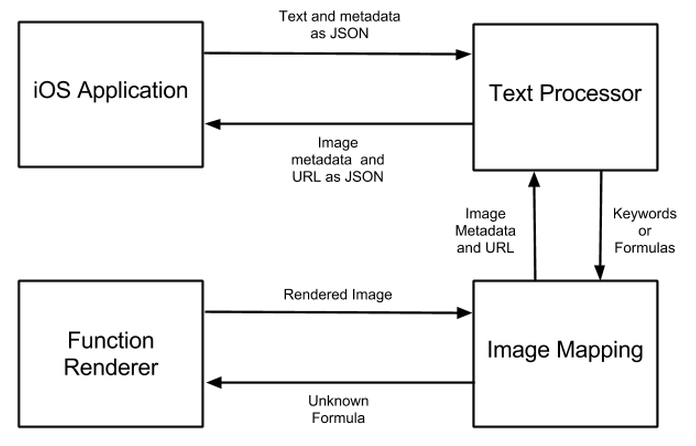
\includegraphics[width=0.9\linewidth]{block_diagram}
	\end{center}
	\vspace{-12pt}
	\caption{Block diagram of our system}
	\label{fig:some_graph}
\end{figure}

\subsection{Technical Challenges}
\label{subsec:tech_challenges}

The most significant technical challenge we will face is defining the rules for detecting each type of code smell. This is more a research problem than an implementation problem, and we will have to perform a series of experiments to fine-tune our detection algorithms. This will be especially difficult because in some cases, we will not have an existing detector to compare results with, but we can overcome this by comparing with human detection. While we are iterating over the source code tokens, we can tweak what generic patterns we look for in order to improve detection. We will have to test multiple patterns to see which works best for each code smell.

We must then determine the best combination of feasible analyses that will yield an accurate and comprehensive reflection of internal code quality. This problem has been attempted many times. The solutions do not work because they are often limited to analyzing single specific factor instead of providing a general assessment of talent. We hope to combine human and machine intelligence using crowdsourcing and machine learning to address this problem, but this strategy will present another challenge in terms of filtering through the results and incorporating them into our model efficiently and correctly.

Another technical challenge will be to determine the optimal weights for each of our code smells when computing the CodeScore. This will be difficult because we will have to analyze user surveys to see which code smells matter more. We will have to determine which machine learning approach will give us the most accurate weights for our metrics. 

Additionally, we have to learn how to parse source code effectively. This is crucial to our project since we are going to need to analyze code not only at a character by character level, but also at a logical level. We need to devise a way to calculate all of our metrics without having to jump around too much in the source code itself. Otherwise, our application would take a long time to execute.

Depending on the way we conduct our crowdsourcing component, another technical challenge may be to standardize all the data that we get from this experiment. To feed this data through our machine learning algorithms, we will need to have discrete variables. This may not be possible if we let users answer questions in an open way. This may limit the kind of data that we can collect from users. Finding out how to achieve a good balance between standardized responses and open ended responses as well as analyzing them will be a challenge.

\subsection{Evaluation Criteria}
\label{subsec:eval_criteria}

Since our project aims to quantitatively analyze code quality to, our evaluation criteria will revolve around checking how accurate our algorithm is in detecting this. We aim to test:

\begin{itemize}
\item How accurately we detect code smells.
\item How accurate our analysis is when compared to human analysis.
\end{itemize}

We hope that by measuring across these three areas, we will be able to validate that our application works as expected. As a goal for the project, we hope to hit 75\% accuracy rates on the first two criteria and hope to beat human analysis at least 50\% of the time.

For the detection of code smells, we can use precision (fraction of detected problems that are really problems) and recall (fraction of problems that are detected) to evaluate the performance. Our goal will be to achieve at least 90\% for both precision and recall with each code smell detector. To do this test systematically, we will feed code through our application that has a fixed number of code smells. For example, we feed in a piece of software that has a total of 10 code smells and check how many code smells our algorithm detects. We have to test for false positives and false negatives. In both these cases, it will imply that our algorithm is not accurate as it should be. We hope that our application will have a < 10\% rate for false results. 

We will also test the output of our machine learning algorithm to see if the various code smells that were found were weighted properly. To this end, we could compute the ``code smell score" by hand and see if it matches the score that was computed by our application. We hope that these figures will always be within 20\% of each other. This way, we can be certain that the output of our machine learning will be used correctly.

The last variant of testing that we can do is human testing. We can give small software packages, comprising of 10 source files each, to both our application and real developers. Our application will compute the CodeScore as well as all of the other metrics about the code. Real developers will then use their best judgement to analyze the code and assign each of the project's CodeScores based on how they found code smells and how they impacted code quality. Our goal is to get to a point where the discrepancy between the CodeScores generated by our application and the real developers happens only 25\% of the time or less. To phrase it differently, we hope that at least 75\% of the time, there will be a rough match between the computed CodeScores. (Rough match is determined by +/- 5\%)
\section{Research Timeline}
\label{sec:research_timeline}
\begin{itemize*}
	\item {\sc already completed}: Performed research on measuring internal code quality. Began looking into parsing techniques for source code and detecting code smells.\vspace{3pt}
	\item {\sc prior to thanksgiving} : Have a basic worker class and controller running. The controller should be able to spawn off workers when the server-side repo is updated.\vspace{3pt}
	\item {\sc prior to christmas} : Have worker class implemented. Should be able to detect code smells and report back to controller. Controller should be able to reduce the output.\vspace{3pt}
\item {\sc by the start of spring term} : Have sample code snippets made for MTurk.\vspace{3pt}	
\item {\sc by the end of march} : Should have results from MTurk experiments. Implement some form of machine learning so that we can analyze the results.\vspace{3pt}
\item {\sc reach goals} : Investigate how to change design to map reduce. Look for more code metrics to measure and incorporate. Add additional code smells. \vspace{3pt}
\item {\sc completion tasks} : Verify implementation meets requirements. Conduct testing mentioned in evaluation section. Complete write-up.\vspace{3pt}
\end{itemize*}

% We next move onto the bibliography.
\bibliographystyle{plain} % Please do not change the bib-style
\bibliography{prop_spec}  % Just the *.BIB filename

% Here is a dirty hack. We insert so much vertical space that the
% appendices, which want to begin in the left colunm underneath
% "references", are pushed over to the right-hand column. If we looked
% hard enough, there is probably a command to do exactly this (and
% wouldn't need tweaked after edits).
\vspace{175pt}

% We then use appendices to share some additional information with
% you, though you won't need appendices in your own proposal.

% The usage of 'enumerate' (similar to 'itemize') we talked about
% above

% You may also notice we have many 'vspace' commands lying
% around. These create 'vertical space' and are a way to force LaTeX
% to cooperate, sometimes. Don't get too involved with using them
% initially, though, because adding or deleting a single line of task
% can dramatically change how LaTeX chooses to format, page, and space
% the document
\end{document} 

